% answers.tex —— 1958 年·广东卷 · 参考答案与详细解析片段
% 由 tools/generate_projects.py 依来源总账自 1958/1958_广东_数学真题_试题.md + 1958/1958_广东_数学真题_解析正文.md + 1958/1958_广东_数学真题_答案要点.md 生成，勿手改（改源 MD 后重跑）


\begin{gktip}
本卷题面出自固定原卷，原卷本身即附有解答；以下解析依据同一材料独立复算表述，不逐字照抄原卷解法。原卷仅第一节（第 1–5 题）以阿拉伯数字编号，其后各大题（第 6–9 题）在原卷中只以中文数字「二、三、四、五」分节、未单独编号，本库按序连续编号以便索引。
\end{gktip}

\gkpart{一}

\begin{answer}
\gksolhead{1}{}

\textbf{题目}：

求二项式 $(3+2x)^5$ 展开式中 $x^3$ 的系数。

\Needspace{4\baselineskip}
\textbf{解析}

\Needspace{5\baselineskip}
二项式 $(3+2x)^5$ 的通项为

\nopagebreak[4]
\[
T_{k+1}=C_5^k\,3^{5-k}(2x)^k=C_5^k\,3^{5-k}2^k\,x^k\qquad(k=0,1,\dots,5)
\]

\Needspace{5\baselineskip}
令 $x$ 的指数 $k=3$，得 $x^3$ 项的系数为

\nopagebreak[4]
\[
C_5^3\cdot3^2\cdot2^3=10\times9\times8=720
\]

\gkanswer{答案：$720$}

\end{answer}
\begin{answer}
\gksolhead{2}{}

\textbf{题目}：

\Needspace{5\baselineskip}
求证：

\nopagebreak[4]
\[
\cos x\cdot\cos 2x\cdot\cos 4x=\frac{\sin 8x}{8\sin x}\qquad(x\ne k\pi,\ k\ \text{为任意整数})
\]

\Needspace{4\baselineskip}
\textbf{解析}

\Needspace{5\baselineskip}
因 $x\ne k\pi$，$\sin x\ne0$，右式恒有意义。反复利用倍角公式 $\sin2\theta=2\sin\theta\cos\theta$：

\nopagebreak[4]
\[
8\sin x\cos x\cdot\cos2x\cdot\cos4x
=4(2\sin x\cos x)\cos2x\cos4x
=4\sin2x\cos2x\cos4x
\]

\nopagebreak[4]
\[
=2(2\sin2x\cos2x)\cos4x=2\sin4x\cos4x=\sin8x
\]

\Needspace{5\baselineskip}
即 $8\sin x\cdot(\cos x\cos2x\cos4x)=\sin8x$。两边除以 $8\sin x$（非零）得

\nopagebreak[4]
\[
\cos x\cdot\cos2x\cdot\cos4x=\frac{\sin8x}{8\sin x}
\]

\gkanswer{答案：见解析版}

\end{answer}
\begin{answer}
\gksolhead{3}{}

\textbf{题目}：

$AB$、$AC$ 为 $\odot O$ 的两弦，$D$ 为 $\widehat{AB}$ 的中点，$E$ 为 $\widehat{AC}$ 的中点，连 $D$、$E$ 交 $AB$ 于 $M$，交 $AC$ 于 $N$。求证：$AM=AN$。
\nopagebreak[4]
\begin{center}% 1958 年广东卷第 3 题：⊙O 中弦 AB、AC，D 为弧 AB 中点、E 为弧 AC 中点，DE 交 AB 于 M、交 AC 于 N（按源卷布局）
\begin{tikzpicture}[scale=1.05, line width=0.45pt,
  every node/.style={inner sep=1.5pt}]
  \coordinate (O) at (0,0);
  \coordinate (A) at (-1.6,0);
  \coordinate (D) at (-0.55,1.5);
  \coordinate (E) at (-0.55,-1.5);
  \coordinate (B) at (1.13,1.13);
  \coordinate (C) at (1.13,-1.13);
  \coordinate (M) at (-0.55,0.44);
  \coordinate (N) at (-0.55,-0.44);
  \draw (O) circle (1.6);
  \draw (D) -- (E);
  \draw (A) -- (B);
  \draw (A) -- (C);
  \fill (A) circle (1.3pt);
  \fill (B) circle (1.3pt);
  \fill (C) circle (1.3pt);
  \fill (D) circle (1.3pt);
  \fill (E) circle (1.3pt);
  \fill (O) circle (1pt);
  \node[anchor=east] at (A) {$A$};
  \node[anchor=south] at (D) {$D$};
  \node[anchor=north] at (E) {$E$};
  \node[anchor=south west] at (B) {$B$};
  \node[anchor=north west] at (C) {$C$};
  \node[anchor=south west] at (M) {$M$};
  \node[anchor=north west] at (N) {$N$};
  \node[anchor=west] at (O) {$O$};
  % 角标 ∠1（M 处）、∠2（N 处），按源图 p-2 所标
  \draw (M) ++(-0.34,0.06) arc (170:262:0.26);
  \node[anchor=east] at ($(M)+(-0.30,0)$) {\tiny$1$};
  \draw (N) ++(-0.34,-0.06) arc (190:98:0.26);
  \node[anchor=east] at ($(N)+(-0.30,0)$) {\tiny$2$};
\end{tikzpicture}
\end{center}
\nopagebreak[4]
\Needspace{4\baselineskip}
\textbf{解析}
\nopagebreak[4]
\begin{center}% 1958 年广东卷第 3 题：⊙O 中弦 AB、AC，D 为弧 AB 中点、E 为弧 AC 中点，DE 交 AB 于 M、交 AC 于 N（按源卷布局）
\begin{tikzpicture}[scale=1.05, line width=0.45pt,
  every node/.style={inner sep=1.5pt}]
  \coordinate (O) at (0,0);
  \coordinate (A) at (-1.6,0);
  \coordinate (D) at (-0.55,1.5);
  \coordinate (E) at (-0.55,-1.5);
  \coordinate (B) at (1.13,1.13);
  \coordinate (C) at (1.13,-1.13);
  \coordinate (M) at (-0.55,0.44);
  \coordinate (N) at (-0.55,-0.44);
  \draw (O) circle (1.6);
  \draw (D) -- (E);
  \draw (A) -- (B);
  \draw (A) -- (C);
  \fill (A) circle (1.3pt);
  \fill (B) circle (1.3pt);
  \fill (C) circle (1.3pt);
  \fill (D) circle (1.3pt);
  \fill (E) circle (1.3pt);
  \fill (O) circle (1pt);
  \node[anchor=east] at (A) {$A$};
  \node[anchor=south] at (D) {$D$};
  \node[anchor=north] at (E) {$E$};
  \node[anchor=south west] at (B) {$B$};
  \node[anchor=north west] at (C) {$C$};
  \node[anchor=south west] at (M) {$M$};
  \node[anchor=north west] at (N) {$N$};
  \node[anchor=west] at (O) {$O$};
  % 角标 ∠1（M 处）、∠2（N 处），按源图 p-2 所标
  \draw (M) ++(-0.34,0.06) arc (170:262:0.26);
  \node[anchor=east] at ($(M)+(-0.30,0)$) {\tiny$1$};
  \draw (N) ++(-0.34,-0.06) arc (190:98:0.26);
  \node[anchor=east] at ($(N)+(-0.30,0)$) {\tiny$2$};
\end{tikzpicture}
\end{center}
\nopagebreak[4]
\Needspace{5\baselineskip}
设直线 $DE$ 与 $AB$ 交于 $M$，与 $AC$ 交于 $N$（如图）。由「圆内角等于其所夹两弧度数和的一半」（两弦相交所成的角）：

\nopagebreak[4]
\[
\angle AMD=\frac12\left(\widehat{AE}+\widehat{BD}\right),\qquad
\angle AND=\frac12\left(\widehat{AD}+\widehat{EC}\right)
\]

\Needspace{5\baselineskip}
（此二角即图中所标 $\angle1$、$\angle2$，与其对顶角度数相同。）因 $D$、$E$ 分别为 $\widehat{AB}$、$\widehat{AC}$ 的中点，有

\nopagebreak[4]
\[
\widehat{AD}=\widehat{BD},\qquad \widehat{AE}=\widehat{EC}
\]

\Needspace{5\baselineskip}
代入得

\nopagebreak[4]
\[
\angle AMD=\frac12\left(\widehat{AE}+\widehat{BD}\right)=\frac12\left(\widehat{EC}+\widehat{AD}\right)=\angle AND
\]

\Needspace{5\baselineskip}
即 $\angle AMN=\angle ANM$（$\angle AMD$、$\angle AND$ 分别与 $\angle AMN$、$\angle ANM$ 互为对顶角或同角）。故 $\triangle AMN$ 中两底角相等，为等腰三角形，从而

\nopagebreak[4]
\[
AM=AN
\]

\gkanswer{答案：见解析版}

\end{answer}
\begin{answer}
\gksolhead{4}{}

\textbf{题目}：

求证：正四面体相对的两棱互相垂直。
\nopagebreak[4]
\begin{center}% 1958 年广东卷第 4 题：正四面体 ABCD，O' 为顶点 A 在底面 BCD 内的射影（按源卷布局；解析正文中记作 O，图中原卷标作 O'，转录保留原卷写法）
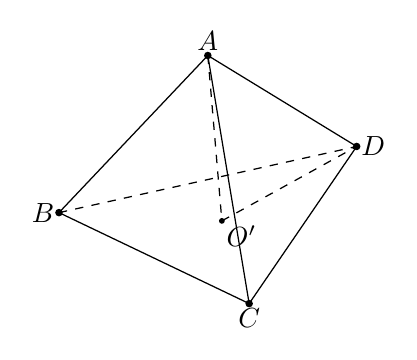
\begin{tikzpicture}[scale=1.05, line width=0.45pt,
  every node/.style={inner sep=1.5pt}]
  \coordinate (A) at (0,1.6);
  \coordinate (B) at (-1.8,-0.3);
  \coordinate (C) at (0.5,-1.4);
  \coordinate (D) at (1.8,0.5);
  \coordinate (Op) at (0.17,-0.4);
  \draw (A) -- (B);
  \draw (A) -- (C);
  \draw (A) -- (D);
  \draw (B) -- (C);
  \draw (C) -- (D);
  \draw[dashed] (B) -- (D);
  \draw[dashed] (A) -- (Op);
  \draw[dashed] (Op) -- (D);
  \fill (A) circle (1.3pt);
  \fill (B) circle (1.3pt);
  \fill (C) circle (1.3pt);
  \fill (D) circle (1.3pt);
  \fill (Op) circle (1pt);
  \node[anchor=south] at (A) {$A$};
  \node[anchor=east] at (B) {$B$};
  \node[anchor=north] at (C) {$C$};
  \node[anchor=west] at (D) {$D$};
  \node[anchor=north west] at (Op) {$O'$};
\end{tikzpicture}
\end{center}
\nopagebreak[4]
\Needspace{4\baselineskip}
\textbf{解析}
\nopagebreak[4]
\begin{center}% 1958 年广东卷第 4 题：正四面体 ABCD，O' 为顶点 A 在底面 BCD 内的射影（按源卷布局；解析正文中记作 O，图中原卷标作 O'，转录保留原卷写法）
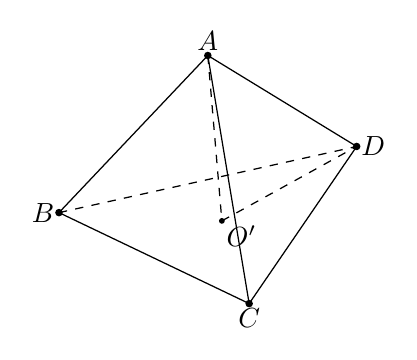
\begin{tikzpicture}[scale=1.05, line width=0.45pt,
  every node/.style={inner sep=1.5pt}]
  \coordinate (A) at (0,1.6);
  \coordinate (B) at (-1.8,-0.3);
  \coordinate (C) at (0.5,-1.4);
  \coordinate (D) at (1.8,0.5);
  \coordinate (Op) at (0.17,-0.4);
  \draw (A) -- (B);
  \draw (A) -- (C);
  \draw (A) -- (D);
  \draw (B) -- (C);
  \draw (C) -- (D);
  \draw[dashed] (B) -- (D);
  \draw[dashed] (A) -- (Op);
  \draw[dashed] (Op) -- (D);
  \fill (A) circle (1.3pt);
  \fill (B) circle (1.3pt);
  \fill (C) circle (1.3pt);
  \fill (D) circle (1.3pt);
  \fill (Op) circle (1pt);
  \node[anchor=south] at (A) {$A$};
  \node[anchor=east] at (B) {$B$};
  \node[anchor=north] at (C) {$C$};
  \node[anchor=west] at (D) {$D$};
  \node[anchor=north west] at (Op) {$O'$};
\end{tikzpicture}
\end{center}
\nopagebreak[4]
\begin{gktip}
\textbf{源注}：原卷正文推导中把顶点 $A$ 在底面内的射影记作 $O$，插图中标作 $O'$；本解析取图中记号 $O'$，二者指同一点，转录保留原卷两处写法的差异。
\end{gktip}

\Needspace{5\baselineskip}
设正四面体 $ABCD$ 的顶点 $A$ 在底面 $\triangle BCD$ 内的射影为 $O'$。因 $\triangle BCD$ 是正三角形，$O'$ 即其中心，连线 $DO'$ 恰是过顶点 $D$ 的中线，同时也是 $BC$ 边上的高，故

\nopagebreak[4]
\[
DO'\perp BC
\]

\Needspace{5\baselineskip}
棱 $AD$ 在底面内的射影即为 $DO'$。由三垂线定理（斜线的射影与平面内一直线垂直，则斜线本身也与该直线垂直），得

\nopagebreak[4]
\[
AD\perp BC
\]

同理，$BO'$ 是 $\triangle BCD$ 过顶点 $B$ 的中线，亦是 $CD$ 边上的高，$BO'\perp CD$，由三垂线定理得 $AB\perp CD$；$CO'$ 是过顶点 $C$ 的中线，亦是 $BD$ 边上的高，$CO'\perp BD$，同理得 $AC\perp BD$。

综上，正四面体相对的三组对棱 $AD$ 与 $BC$、$AB$ 与 $CD$、$AC$ 与 $BD$ 均互相垂直。

\gkanswer{答案：见解析版}

\end{answer}
\begin{answer}
\gksolhead{5}{}

\textbf{题目}：

解方程 $\sin x=\sqrt3\cos x$。

\Needspace{4\baselineskip}
\textbf{解析}

\Needspace{5\baselineskip}
方程 $\sin x=\sqrt3\cos x$ 中，若 $\cos x=0$ 则须 $\sin x=0$，与 $\sin^2x+\cos^2x=1$ 矛盾，故 $\cos x\ne0$，两边同除 $\cos x$：

\nopagebreak[4]
\[
\tan x=\sqrt3
\]

\Needspace{5\baselineskip}
因 $\tan\dfrac\pi3=\sqrt3$ 且正切函数周期为 $\pi$，故

\nopagebreak[4]
\[
x=\frac\pi3+k\pi\qquad(k\in\mathbb Z)
\]

\gkanswer{答案：$x=k\pi+\dfrac\pi3$（$k\in\mathbb Z$）}

\end{answer}
\gkpart{二}

\begin{answer}
\gksolhead{6}{}

\textbf{题目}：

\Needspace{5\baselineskip}
解方程组：

\nopagebreak[4]
\[
\begin{cases}
\sqrt{x+\dfrac1y}+\sqrt{x+2y-1}=4,\\[4pt]
2x+2y+\dfrac1y=9.
\end{cases}
\]

\Needspace{4\baselineskip}
\textbf{解析}

\Needspace{5\baselineskip}
设 $X=\sqrt{x+\dfrac1y}\ (\ge0)$，$Y=\sqrt{x+2y-1}\ (\ge0)$。原方程组的第一式即

\nopagebreak[4]
\[
X+Y=4\tag{1}
\]

\Needspace{5\baselineskip}
第二式可改写：

\nopagebreak[4]
\[
X^2+Y^2=\left(x+\frac1y\right)+(x+2y-1)=\left(2x+2y+\frac1y\right)-1=9-1=8\tag{2}
\]

\Needspace{5\baselineskip}
由 $(1)^2$：$X^2+2XY+Y^2=16$，结合 (2) 得 $2XY=16-8=8$，即 $XY=4$。于是 $X$、$Y$ 是方程 $t^2-4t+4=0$ 的两根，即 $(t-2)^2=0$，故

\nopagebreak[4]
\[
X=Y=2
\]

\Needspace{5\baselineskip}
代回定义：

\nopagebreak[4]
\[
x+\frac1y=4\tag{3}
\]

\nopagebreak[4]
\[
x+2y-1=4\tag{4}
\]

$(4)-(3)$：$2y-\dfrac1y=1$，即 $2y^2-y-1=0$，因式分解 $(2y+1)(y-1)=0$，得 $y=1$ 或 $y=-\dfrac12$。

代入 (3)：$y=1$ 时 $x=4-1=3$；$y=-\dfrac12$ 时 $x=4-(-2)=6$。

\Needspace{5\baselineskip}
两组解均使 $X=Y=2\ge0$、$x+\dfrac1y=4\ge0$、$x+2y-1=4\ge0$，与原方程组相容，经检验均为原方程组的解：

\nopagebreak[4]
\[
\begin{cases}x=3\\y=1\end{cases}\qquad\text{或}\qquad\begin{cases}x=6\\y=-\dfrac12\end{cases}
\]

\gkanswer{答案：$\begin{cases}x=3\\y=1\end{cases}$ 或 $\begin{cases}x=6\\y=-\dfrac12\end{cases}$}

\end{answer}
\gkpart{三}

\begin{answer}
\gksolhead{7}{}

\textbf{题目}：

设有两个同心圆，半径各为 $R$、$r$（$R>r$）。今由圆心 $O$ 作半径交大圆于 $A$，交小圆于 $A'$，由 $A$ 作直线 $AD$ 垂直于大圆直径 $BC$，并交 $BC$ 于 $D$，作 $A'E\perp AD$，并交 $AD$ 于 $E$。

已知：$\angle OAD=\alpha$。

求：$OE$ 的长。
\nopagebreak[4]
\begin{center}% 1958 年广东卷第 7 题：同心圆 O（半径 R、r），半径 OA 交大圆于 A、交小圆于 A'，AD⊥BC 于 D，A'D'⊥BC 于 D'，A'E⊥AD 于 E（按源卷布局）
\begin{tikzpicture}[scale=1.0, line width=0.45pt,
  every node/.style={inner sep=1.5pt}]
  \coordinate (O) at (0,0);
  \coordinate (B) at (0,2);
  \coordinate (C) at (0,-2);
  \coordinate (D) at (0,-1.148);
  \coordinate (Dp) at (0,-0.631);
  \coordinate (A) at (-1.638,-1.148);
  \coordinate (Ap) at (-0.901,-0.631);
  \coordinate (E) at (-0.901,-1.148);
  \draw (O) circle (2);
  \draw (O) circle (1.1);
  \draw (B) -- (C);
  \draw (A) -- (D);
  \draw (O) -- (A);
  \draw (O) -- (E);
  \draw (Ap) -- (D);
  \draw[dashed] (Ap) -- (Dp);
  \draw (Ap) -- (E);
  \draw (A) ++(0:0.32) arc (0:35:0.32);
  \draw (Ap) ++(0:0.18) arc (0:35:0.18);
  \node[anchor=west] at ($(A)+(17:0.48)$) {$\alpha$};
  \node[anchor=south west] at ($(Ap)+(17:0.3)$) {\tiny$\alpha$};
  \fill (O) circle (1pt);
  \fill (A) circle (1.3pt);
  \fill (Ap) circle (1.3pt);
  \fill (D) circle (1.3pt);
  \fill (Dp) circle (1.3pt);
  \fill (E) circle (1.3pt);
  \fill (B) circle (1.3pt);
  \fill (C) circle (1.3pt);
  \node[anchor=south] at (B) {$B$};
  \node[anchor=north] at (C) {$C$};
  \node[anchor=east] at (O) {$O$};
  \node[anchor=north west] at (D) {$D$};
  \node[anchor=south west] at (Dp) {$D'$};
  \node[anchor=east] at (A) {$A$};
  \node[anchor=south east] at (Ap) {$A'$};
  \node[anchor=north] at (E) {$E$};
\end{tikzpicture}
\end{center}
\nopagebreak[4]
\Needspace{4\baselineskip}
\textbf{解析}
\nopagebreak[4]
\begin{center}% 1958 年广东卷第 7 题：同心圆 O（半径 R、r），半径 OA 交大圆于 A、交小圆于 A'，AD⊥BC 于 D，A'D'⊥BC 于 D'，A'E⊥AD 于 E（按源卷布局）
\begin{tikzpicture}[scale=1.0, line width=0.45pt,
  every node/.style={inner sep=1.5pt}]
  \coordinate (O) at (0,0);
  \coordinate (B) at (0,2);
  \coordinate (C) at (0,-2);
  \coordinate (D) at (0,-1.148);
  \coordinate (Dp) at (0,-0.631);
  \coordinate (A) at (-1.638,-1.148);
  \coordinate (Ap) at (-0.901,-0.631);
  \coordinate (E) at (-0.901,-1.148);
  \draw (O) circle (2);
  \draw (O) circle (1.1);
  \draw (B) -- (C);
  \draw (A) -- (D);
  \draw (O) -- (A);
  \draw (O) -- (E);
  \draw (Ap) -- (D);
  \draw[dashed] (Ap) -- (Dp);
  \draw (Ap) -- (E);
  \draw (A) ++(0:0.32) arc (0:35:0.32);
  \draw (Ap) ++(0:0.18) arc (0:35:0.18);
  \node[anchor=west] at ($(A)+(17:0.48)$) {$\alpha$};
  \node[anchor=south west] at ($(Ap)+(17:0.3)$) {\tiny$\alpha$};
  \fill (O) circle (1pt);
  \fill (A) circle (1.3pt);
  \fill (Ap) circle (1.3pt);
  \fill (D) circle (1.3pt);
  \fill (Dp) circle (1.3pt);
  \fill (E) circle (1.3pt);
  \fill (B) circle (1.3pt);
  \fill (C) circle (1.3pt);
  \node[anchor=south] at (B) {$B$};
  \node[anchor=north] at (C) {$C$};
  \node[anchor=east] at (O) {$O$};
  \node[anchor=north west] at (D) {$D$};
  \node[anchor=south west] at (Dp) {$D'$};
  \node[anchor=east] at (A) {$A$};
  \node[anchor=south east] at (Ap) {$A'$};
  \node[anchor=north] at (E) {$E$};
\end{tikzpicture}
\end{center}
\nopagebreak[4]
\Needspace{5\baselineskip}
在直角 $\triangle OAD$ 中（$AD\perp BC$ 于 $D$，$OD$ 是 $BC$ 上的一段，故 $\angle ODA=90^\circ$），斜边 $OA=R$，$\angle OAD=\alpha$，故

\nopagebreak[4]
\[
OD=OA\sin\alpha=R\sin\alpha,\qquad AD=OA\cos\alpha=R\cos\alpha
\]

\Needspace{5\baselineskip}
同理，因 $A'$ 在半径 $OA$ 上且 $OA'=r$，若设 $D'$ 为 $A'$ 在 $BC$ 上的垂足，则 $\triangle OA'D'$ 与 $\triangle OAD$ 相似（比例 $r:R$），故

\nopagebreak[4]
\[
OD'=r\sin\alpha,\qquad A'D'=r\cos\alpha
\]

\Needspace{5\baselineskip}
又 $AA'=OA-OA'=R-r$，且 $\angle A'AE=\angle OAD=\alpha$（同一直线 $OA$ 上的角），$A'E\perp AD$，故在直角 $\triangle A'AE$ 中

\nopagebreak[4]
\[
AE=AA'\cos\alpha=(R-r)\cos\alpha
\]

\Needspace{5\baselineskip}
于是

\nopagebreak[4]
\[
ED=AD-AE=R\cos\alpha-(R-r)\cos\alpha=r\cos\alpha
\]

\Needspace{5\baselineskip}
在直角 $\triangle OED$ 中（$OD\perp ED$，因 $OD$ 沿 $BC$ 方向、$ED$ 沿 $AD$ 方向，两方向互相垂直），由勾股定理：

\nopagebreak[4]
\[
OE=\sqrt{OD^2+ED^2}=\sqrt{R^2\sin^2\alpha+r^2\cos^2\alpha}
\]

\gkanswer{答案：$OE=\sqrt{R^2\sin^2\alpha+r^2\cos^2\alpha}$}

\end{answer}
\gkpart{四}

\begin{answer}
\gksolhead{8}{}

\textbf{题目}：

已知 $\triangle ABC$，求作圆过 $A$ 及 $AB$ 中点 $M$，并与 $BC$ 相切。
\nopagebreak[4]
\begin{center}% 1958 年广东卷第 8 题：△ABC 中过 A、AB 中点 M 且与 BC 相切于 T 的圆 O；辅助半圆（直径 AD，BD=BM，BE⊥AD 于 B，用以作比例中项 BE）（按源卷布局）
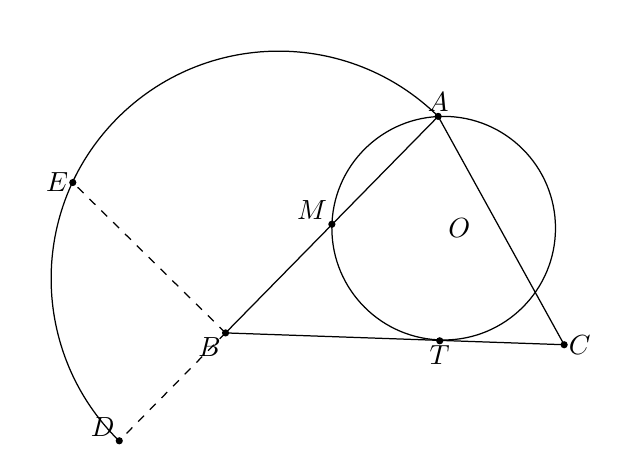
\begin{tikzpicture}[scale=1.0, line width=0.45pt,
  every node/.style={inner sep=1.5pt}]
  \coordinate (A) at (2.70,2.75);
  \coordinate (B) at (0,0);
  \coordinate (C) at (4.30,-0.15);
  \coordinate (M) at (1.35,1.38);
  \coordinate (O) at (2.77,1.33);
  \coordinate (T) at (2.72,-0.10);
  \coordinate (D) at (-1.35,-1.37);
  \coordinate (E) at (-1.94,1.91);
  \draw (A) -- (B) -- (C) -- cycle;
  \draw (O) circle (1.42);
  \draw[dashed] (B) -- (E);
  \draw[dashed] (B) -- (D);
  \draw (A) arc (45.5:225.5:2.89);
  \fill (A) circle (1.3pt);
  \fill (B) circle (1.3pt);
  \fill (C) circle (1.3pt);
  \fill (M) circle (1.3pt);
  \fill (T) circle (1.3pt);
  \fill (D) circle (1.3pt);
  \fill (E) circle (1.3pt);
  \node[anchor=south] at (A) {$A$};
  \node[anchor=north east] at (B) {$B$};
  \node[anchor=west] at (C) {$C$};
  \node[anchor=south east] at (M) {$M$};
  \node[anchor=west] at (O) {$O$};
  \node[anchor=north] at (T) {$T$};
  \node[anchor=south east] at (D) {$D$};
  \node[anchor=east] at (E) {$E$};
\end{tikzpicture}
\end{center}
\nopagebreak[4]
\Needspace{4\baselineskip}
\textbf{解析}
\nopagebreak[4]
\begin{center}% 1958 年广东卷第 8 题：△ABC 中过 A、AB 中点 M 且与 BC 相切于 T 的圆 O；辅助半圆（直径 AD，BD=BM，BE⊥AD 于 B，用以作比例中项 BE）（按源卷布局）
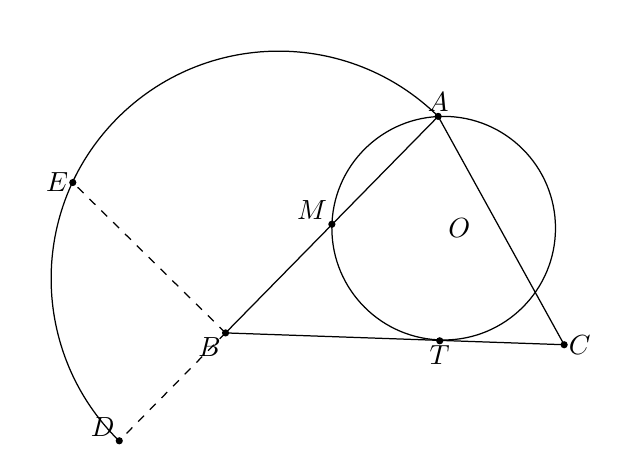
\begin{tikzpicture}[scale=1.0, line width=0.45pt,
  every node/.style={inner sep=1.5pt}]
  \coordinate (A) at (2.70,2.75);
  \coordinate (B) at (0,0);
  \coordinate (C) at (4.30,-0.15);
  \coordinate (M) at (1.35,1.38);
  \coordinate (O) at (2.77,1.33);
  \coordinate (T) at (2.72,-0.10);
  \coordinate (D) at (-1.35,-1.37);
  \coordinate (E) at (-1.94,1.91);
  \draw (A) -- (B) -- (C) -- cycle;
  \draw (O) circle (1.42);
  \draw[dashed] (B) -- (E);
  \draw[dashed] (B) -- (D);
  \draw (A) arc (45.5:225.5:2.89);
  \fill (A) circle (1.3pt);
  \fill (B) circle (1.3pt);
  \fill (C) circle (1.3pt);
  \fill (M) circle (1.3pt);
  \fill (T) circle (1.3pt);
  \fill (D) circle (1.3pt);
  \fill (E) circle (1.3pt);
  \node[anchor=south] at (A) {$A$};
  \node[anchor=north east] at (B) {$B$};
  \node[anchor=west] at (C) {$C$};
  \node[anchor=south east] at (M) {$M$};
  \node[anchor=west] at (O) {$O$};
  \node[anchor=north] at (T) {$T$};
  \node[anchor=south east] at (D) {$D$};
  \node[anchor=east] at (E) {$E$};
\end{tikzpicture}
\end{center}
\nopagebreak[4]
\textbf{作法}：延长 $AB$ 至 $D$，使 $BD=\dfrac{AB}2=BM$；以 $AD$ 为直径作半圆，过 $B$ 作 $AD$ 的垂线，交半圆于 $E$；在 $BC$ 上截取 $BT=BE$；过 $A$、$M$、$T$ 三点作圆，即为所求。

\Needspace{5\baselineskip}
\textbf{证明}：因 $AD$ 是所作半圆的直径，$E$ 在半圆上，由「直径所对的圆周角是直角」得 $\angle AED=90^\circ$。在直角 $\triangle AED$ 中，$EB$ 是斜边 $AD$ 上的高（$EB\perp AD$ 于 $B$），由射影定理（直角三角形斜边上的高是两直角边在斜边上射影的比例中项）：

\nopagebreak[4]
\[
BE^2=BD\cdot BA
\]

\Needspace{5\baselineskip}
又作图时取 $BD=BM$，故

\nopagebreak[4]
\[
BT^2=BE^2=BD\cdot BA=BM\cdot BA
\]

由切割线定理的逆命题：若由圆外一点 $B$ 引一条直线交圆于 $M$、$A$ 两点，另一射线交圆于 $T$，且 $BT^2=BM\cdot BA$，则该射线在 $T$ 处与圆相切。此处 $T$ 恰满足 $BT^2=BM\cdot BA$，故 $BC$ 在 $T$ 处与过 $A$、$M$、$T$ 的圆相切，即所作的圆过 $A$、$AB$ 中点 $M$，且与 $BC$ 相切，为所求。

\gkanswer{答案：见解析版}

\end{answer}
\gkpart{五}

\begin{answer}
\gksolhead{9}{}

\textbf{题目}：

\Needspace{5\baselineskip}
已知一直角三角形的斜边长为 $2$，斜边上的高为 $\dfrac{\sqrt3}{2}$，求证：此三角形的两个锐角是下列三角方程的根：

\nopagebreak[4]
\[
\sin^2x-\frac{1+\sqrt3}{2}\sin x+\frac{\sqrt3}{4}=0
\]
\nopagebreak[4]
\begin{center}% 1958 年广东卷第 9 题：直角三角形，斜边 2，斜边上的高 √3/2，两腰记 a、b，右侧锐角记 α（按源卷布局）
\begin{tikzpicture}[scale=1.6, line width=0.45pt,
  every node/.style={inner sep=1.5pt}]
  \coordinate (L) at (0,0);
  \coordinate (R) at (2,0);
  \coordinate (F) at (0.5,0);
  \coordinate (P) at (0.5,0.866);
  \draw (L) -- (R) -- (P) -- cycle;
  \draw (P) -- (F);
  \draw (F) ++(0,0.08) -- ++(0.08,0) -- ++(0,-0.08);
  \node[anchor=south east] at (0.14,0.50) {$a$};
  \node[anchor=west] at ($(P)!0.5!(R)$) {$b$};
  \node[anchor=north] at ($(L)!0.5!(R)$) {$2$};
  \node[anchor=west] at (0.56,0.42) {$\dfrac{\sqrt3}{2}$};
  \node[anchor=north west] at (1.68,0.05) {$\alpha$};
\end{tikzpicture}
\end{center}
\nopagebreak[4]
\Needspace{4\baselineskip}
\textbf{解析}
\nopagebreak[4]
\begin{center}% 1958 年广东卷第 9 题：直角三角形，斜边 2，斜边上的高 √3/2，两腰记 a、b，右侧锐角记 α（按源卷布局）
\begin{tikzpicture}[scale=1.6, line width=0.45pt,
  every node/.style={inner sep=1.5pt}]
  \coordinate (L) at (0,0);
  \coordinate (R) at (2,0);
  \coordinate (F) at (0.5,0);
  \coordinate (P) at (0.5,0.866);
  \draw (L) -- (R) -- (P) -- cycle;
  \draw (P) -- (F);
  \draw (F) ++(0,0.08) -- ++(0.08,0) -- ++(0,-0.08);
  \node[anchor=south east] at (0.14,0.50) {$a$};
  \node[anchor=west] at ($(P)!0.5!(R)$) {$b$};
  \node[anchor=north] at ($(L)!0.5!(R)$) {$2$};
  \node[anchor=west] at (0.56,0.42) {$\dfrac{\sqrt3}{2}$};
  \node[anchor=north west] at (1.68,0.05) {$\alpha$};
\end{tikzpicture}
\end{center}
\nopagebreak[4]
\Needspace{5\baselineskip}
设直角三角形的一个锐角为 $x$，则另一锐角为 $90^\circ-x$；斜边 $c=2$，两直角边分别为

\nopagebreak[4]
\[
a=c\sin x=2\sin x,\qquad b=c\sin(90^\circ-x)=c\cos x=2\cos x
\]

\Needspace{5\baselineskip}
三角形面积可用两种方式表示。一方面，用两直角边：

\nopagebreak[4]
\[
S=\frac12ab=\frac12(2\sin x)(2\cos x)=2\sin x\cos x=\sin2x
\]

\Needspace{5\baselineskip}
另一方面，用斜边及斜边上的高：

\nopagebreak[4]
\[
S=\frac12\cdot c\cdot h=\frac12\times2\times\frac{\sqrt3}2=\frac{\sqrt3}2
\]

\Needspace{5\baselineskip}
两式相等，得 $\sin2x=\dfrac{\sqrt3}2$，即

\nopagebreak[4]
\[
\sin x\cos x=\frac{\sqrt3}4\tag{1}
\]

\Needspace{5\baselineskip}
又恒有 $\sin^2x+\cos^2x=1$，结合 (1)：

\nopagebreak[4]
\[
(\sin x+\cos x)^2=1+2\sin x\cos x=1+\frac{\sqrt3}2=\frac{2+\sqrt3}2
\]

\Needspace{5\baselineskip}
注意到 $\left(\dfrac{1+\sqrt3}2\right)^2=\dfrac{4+2\sqrt3}4=\dfrac{2+\sqrt3}2$，且 $x$ 为锐角时 $\sin x+\cos x>0$，故

\nopagebreak[4]
\[
\sin x+\cos x=\frac{1+\sqrt3}2\tag{2}
\]

\Needspace{5\baselineskip}
由 (1)、(2) 可知，$\sin x$ 与 $\cos x$ 是以

\nopagebreak[4]
\[
t^2-\frac{1+\sqrt3}2t+\frac{\sqrt3}4=0
\]

\Needspace{5\baselineskip}
为特征方程、和为 $\dfrac{1+\sqrt3}2$、积为 $\dfrac{\sqrt3}4$ 的两个数，即它们都满足此方程。而该直角三角形的两个锐角分别为 $x$、$90^\circ-x$，其正弦依次为 $\sin x$、$\sin(90^\circ-x)=\cos x$，故两锐角的正弦都是方程

\nopagebreak[4]
\[
\sin^2t-\frac{1+\sqrt3}2\sin t+\frac{\sqrt3}4=0
\]

的根，即两个锐角都是题设三角方程的根。

（附：解此二次方程可得 $\sin t=\dfrac12$ 或 $\sin t=\dfrac{\sqrt3}2$，对应两锐角为 $30^\circ$ 与 $60^\circ$；验证 $\sin30^\circ\sin60^\circ=\dfrac12\cdot\dfrac{\sqrt3}2=\dfrac{\sqrt3}4$、$\sin30^\circ+\sin60^\circ=\dfrac12+\dfrac{\sqrt3}2=\dfrac{1+\sqrt3}2$，与上式一致，且以 $30^\circ,60^\circ,90^\circ$ 为内角、斜边 $2$ 的直角三角形，斜边上的高确为 $\dfrac{\sqrt3}2$，与题设相符。）

\gkanswer{答案：见解析版}

\end{answer}